\documentclass[oldfontcommands,oneside,a4paper,11pt]{article} 
\usepackage{fontspec}
\usepackage{natbib}
\usepackage{booktabs}
\usepackage{xltxtra} 
\usepackage{polyglossia} 
\setdefaultlanguage{french} 
\usepackage[table]{xcolor}
\usepackage{multirow}
\usepackage{gb4e} 
\usepackage{graphicx}
\usepackage{float}
\usepackage{lscape}
\usepackage{hyperref} 
\hypersetup{bookmarks=false,bookmarksnumbered,bookmarksopenlevel=5,bookmarksdepth=5,xetex,colorlinks=true,linkcolor=blue,citecolor=blue}
\usepackage[all]{hypcap}
\usepackage{memhfixc}

\bibpunct[~: ]{(}{)}{,}{a}{}{,} 


\setmainfont[Mapping=tex-text,Numbers=OldStyle,Ligatures=Common]{Charis SIL} %ici on définit la police par défaut du texte


\newfontfamily\phon[Mapping=tex-text,Ligatures=Common,Scale=MatchLowercase,FakeSlant=0.3]{Charis SIL}  
\newcommand{\ipa}[1]{{\phon #1}} %API tjs en italique
\newcommand{\ipac}[1]{{\tiny #1}} 
\newfontfamily\cn[Mapping=tex-text,Ligatures=Common,Scale=MatchUppercase]{MingLiU}%pour le chinois
\newcommand{\zh}[1]{{\cn #1}}
\newcommand{\petit}[1]{\tiny#1}
\newcommand{\sig}{\begin{math}\Sigma\end{math}} 
\newcommand{\ra}{$\Sigma_1$} 
\newcommand{\rc}{$\Sigma_3$} 
\newcommand{\grise}[1]{\cellcolor{lightgray}\textbf{#1}}


\begin{document}
%\OnehalfSpacing
\title{Projet de recherche} 
\author{Guillaume Jacques}
\maketitle

\sloppy
\tableofcontents
\section{Grammaire et corpus de référence du japhug}
Ma priorité à moyen terme est de finir une grammaire de référence du japhug, accompagnée d'un dictionnaire et d'un corpus de textes disponibles en ligne. Une première version du dictionnaire sera disponible en ligne d'ici mi-2015, et le corpus sera progressivement publié sur le site Pangloss. 

Ce corpus, qui dépasse 60h de textes enregistrés (sans compter les phrases isolées et les listes de mots), aura besoin d'être complété toutefois par davantage de conversations -- il n'en comprend actuellement seulement que 40 minutes. Or, les conversations, par opposition aux histoires et aux textes procéduraux, sont indispensables pour éclaircir de nombreux aspects de la grammaire, en particulier le TAM et l'usage des particules de fin de phrase. En outre, pour les textes procéduraux, je compte collecter davantage de données vidéo. 

Néanmoins, je considère déjà disposer d'un corpus relativement représentatif pour une description de la langue assez détaillée. C'est donc la rédaction de la grammaire qui est maintenant pour moi la tâche prioritaire.



Si j'ai déjà publié une grammaire en chinois (\citealt{jacques08zh}), celle-ci, du fait des contraintes de la collection où elle a été publiée, est relativement courte (472 pp -- j'avais dû raccourcir le manuscrit) et n'est pas utilisable par les typologues occidentaux à cause de la barrière de la langue. Par ailleurs, ma connaissance du japhug est considérablement plus avancée maintenant qu'en 2006-2007 (lorsque je rédigeais ce livre), et mon corpus actuel est six fois plus long qu'à cette époque. Il est donc indispensable d'écrire une nouvelle grammaire en anglais, destinée aux typologues et aux comparatistes.  Ce travail n'est pas redondant avec la grammaire de 2008, car il s'adresse à une audience différent, et sera basé sur un corpus d'une taille beaucoup plus conséquente.

Depuis 2010, j'ai publié une série d'articles en anglais sur plusieurs points de la morphosyntaxe du japhug, qui peuvent être remaniés comme chapitres de grammaire en ajoutant de nouveaux exemples, en supprimant les redondances et en les intégrant à l'ensemble du manuscrit. Cela inclut les sections sur l'indexation (\citealt{jacques10inverse}), la valence et la voix (\citealt{jacques12demotion}, \citealt{jacques12incorp}, \citealt{jacques13tropative},   \citealt{jacques14antipassive}), les idéophones (\citealt{japhug14ideophones}), le mouvement associé et les constructions à verbe de mouvement (\citealt{jacques13harmonization}) et le chainage de propositions (\citealt{jacques14linking}). Si l'on prend en compte d'autres sections déjà partiellement rédigées, je dispose déjà en tout de 290 pages, mais ces matériaux n'ont pas encore été combinés en un  tout cohérent.

Il reste encore à écrire de nombreuses parties de la grammaire: les sections sur la nominalisation, la complémentation, la morphologie nominale, la structure de la phrase nominale, les classes de verbes, les pivots syntaxiques et l'alignement, les quantificateurs, les particules de fin de phrase, la structure informationnelle, et de compléter celles sur les marques de voix, la dérivation verbale et le TAM.

  J'ai soumis cinq articles qui pourront être intégrés sous forme remaniée à la grammaire sur la phonologie (\textit{illustration of the IPA}), les comparatives, le générique, les constructions causatives et les relatives. Je compte soumettre en 2015 et 2016 au moins cinq articles sur la morphosyntaxe du japhug: les numéraux et les classificateurs (pour un Festschrift), le préfixe spontané / autobénéfactif, le discours indirect hybride, les complétives et l'évidentialité. 
  
  Lorsque tous ces articles seront achevés, je me consacrerai pleinement  à synthétiser toutes les sections déjà rédigées et à les compléter, ainsi qu'à écrire les sections qui peuvent difficilement mener à un article (dans les domaines de la grammaire où le japhug n'est pas typologiquement inhabituel).

J'estime à quatre ans, à raison de 150 pages par an (ajoutées à celles déjà écrites), le délai nécessaire minimal pour compléter la première version complète de la grammaire (pour 2018-2019).

\section{Grammaire comparée des langues rgyalronguiques et des langues kiranti}
La grammaire du japhug sera la première pierre d'un édifice plus général -- la grammaire comparée (synchronique et diachronique) des langues rgyalronguiques et kiranti, les deux branches de la famille sino-tibétaine dont la morphologie verbale est la plus complexe (voir les cartes  \ref{fig:rgy}  et \ref{fig:kirant}). Ces deux branches comprennent respectivement 10 et 22 langues au minimum -- soit une quantité de données plus grande que l'ensemble de la famille algonquienne, et il me semble préférable de concentrer mes efforts sur ces deux groupes plutôt que d'essayer de maîtriser l'ensemble des données sino-tibétaines.

   \begin{figure}[h]
   \caption{Langues rgyalronguiques (Sichuan tibétain) }  \label{fig:rgy}  \centering
 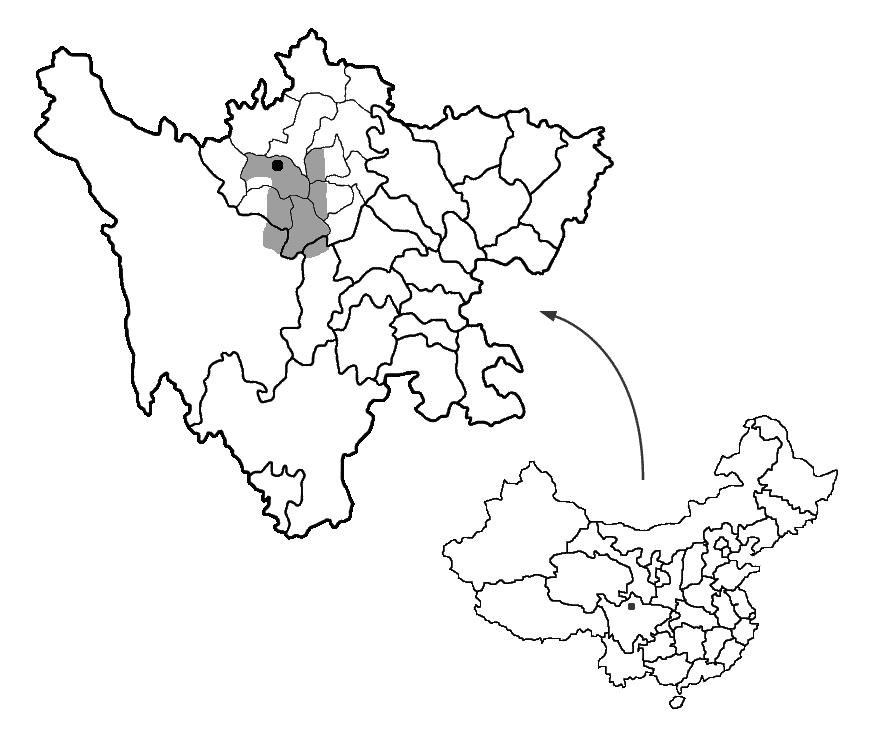
\includegraphics[width=0.6\textwidth]{carte.JPG}
 \end{figure}
Ce projet de recherche sera nécessairement collectif, car la masse des données à traiter rend impraticable une approche isolée. Il comprendra quatre parties: descriptions des langues et collection de données, phonologie comparée du rgyalronguique, phonologie historique du khaling et enfin morphosyntaxe comparée.

 \begin{figure}[h]
   \caption{Langues kiranti (est du Népal)} \label{fig:kirant}   \centering
  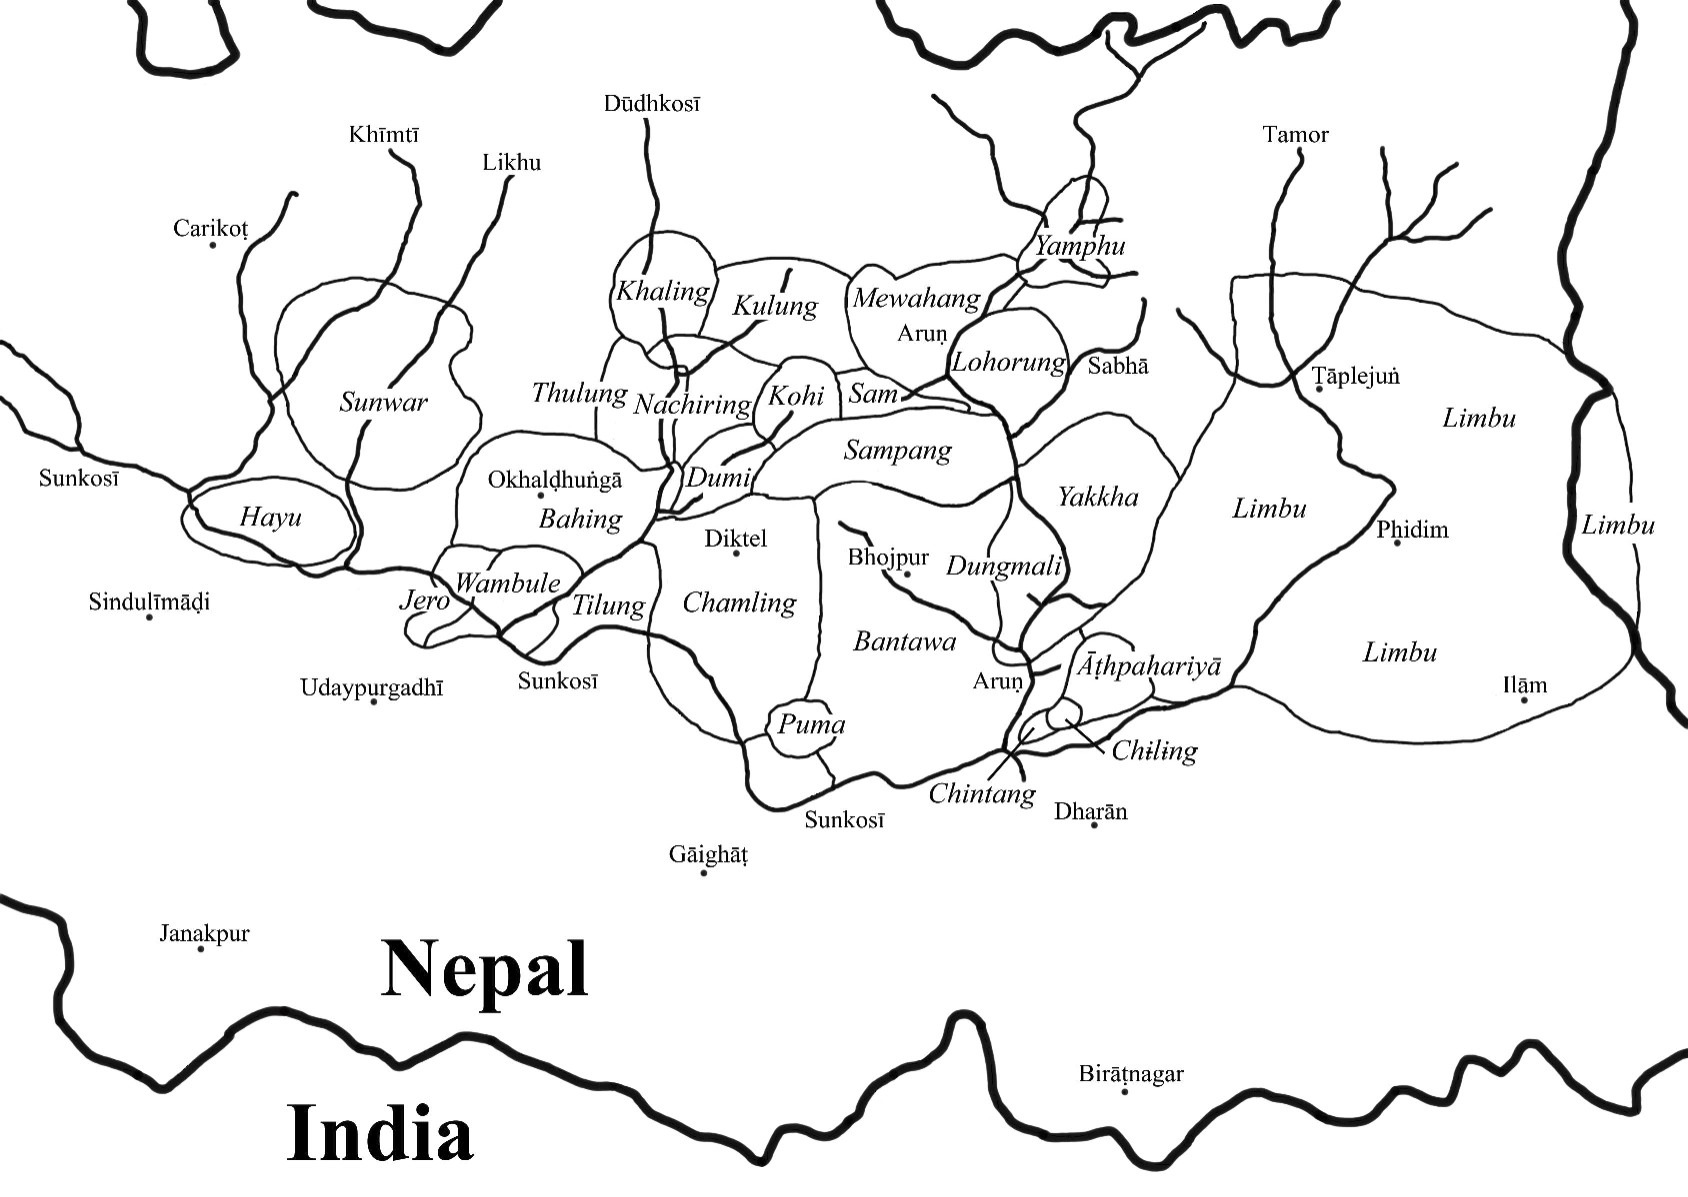
\includegraphics[width=\textwidth]{Kirant.jpeg} 
 \end{figure}
 
\subsection{Collection de données}
Une recherche comparative requiert des données riches, fiables et complètes sur toutes les langues étudiées, et à ce titre cette entreprise n'est pas réalisable sur la base exclusive de la grammaire japhug.

Je ne compte pas d'ici 2020 me charger de rédiger de grammaire autre que celle du japhug. Néanmoins, je continuerai à travailler sur trois autres langues, le khaling, le stau et le situ, collecterai des enregistrements, et écrirai des articles sur des points spécifiques de morphosyntaxe, probablement en collaboration (avec Aimée Lahaussois, Anton Antonov, Lai Yunfan et Gong Xun). Il est probable que certains de ces articles pourront mener à des contributions théoriques plus générales, et conduire notre recherche en typologie dans des directions nouvelles.

En outre, j'envisage un rôle de supervision: diriger des thèses de façon à couvrir l'ensemble des langues (et les dialectes) rgyalronguiques et kiranti qui restent à décrire, ainsi qu'à approfondir des points spécifiques sur les langues mieux dotées. Outre les langues modernes, je compte également former des étudiants en philologie tangoute, qui pourrons prolonger mes travaux et valoriser le corpus que j'ai déjà transcrit dans cette langue. 
 

Je continuerai à enseigner dans le mastaire conjoint Inalco-Paris III afin de découvrir et former les étudiants prometteurs, avant leur formation doctorale et les aider à acquérir rapidement la capacité à rédiger des travaux publiables.

J'espère  fonder une école française de linguistique sino-tibétaine, dont chaque membre devra se charger de la documentation complète (avec corpus d'enregistrements d'au moins une dizaine d'heure, dictionnaire et grammaire) d'une langue rgyalronguique, tibétaine ou  kiranti, mais aussi se former en informatique (Perl/Python, transducteurs, langages formels, \LaTeX, R)  et en linguistique historique (indo-européenne et sino-tibétaine).

Ces trois domaines sont traditionnellement séparés, mais je suis convaincu qu'ils sont complémentaires. La linguistique de terrain permet d'effectuer un travail de description utile à long terme, aide à acquérir la connaissance pratique d'une langue peu connue et rend possible la découverte de phénomènes complètement inconnus. 
 La linguistique informatique est utile pour traiter plus efficacement le corpus transcrit, et automatiser les tâches qui peuvent l'être. D'autre part, la connaissance de la théorie des langages formels et automates permet une approche théorique implémentable  aussi bien en phonologie qu'en morphologie ou qu'en syntaxe.
La linguistique historique, enfin, apporte une dimension explicative qui enrichit l'approche   synchronique et formelle des données.

Outre les langues sino-tibétaines, je développerai aussi les études des langues d'Amérique du nord (en particulier sioux et algonquien) qui sont encore sous-représentées chez les linguistes français.

\subsection{Phonologie et morphologie comparée du rgyalronguique} \label{sec:comparee.rgy}
Dans mes travaux précédents, en particulier \citet{jacques04these} et \citet{jacques14esquisse}, j'ai présenté une reconstruction préliminaire du proto-rgyalrong, et ai établi un certain nombre de lois phonétiques. Toutefois, ces résultats, basés sur des données incomplètes, devront être intégralement revus lorsque, dans cinq à dix ans, on disposera de lexiques fiables sur toutes les langues rgyalronguiques.

Le lexique comparatif des langues rgyalronguiques comprend actuellement plus de 700 groupes de cognats. Etant donné la proximité de ces langues, il sera sans doute possible de doubler le nombre de cognats avec des lexiques plus complets,  d'affiner les lois déjà connues et d'en découvrir de nouvelles. 

Outre la reconstruction phonologique proprement dite, il est nécessaire d'intégrer la morphologie dans ces reconstructions, en particulier les alternances de thèmes verbaux réguliers et irréguliers et les dérivations verbales et dénominales. Si certaines alternances vocaliques peuvent être expliquées comme résultant de la fusion du radical verbal avec des suffixes (\citealt[357-8]{jacques04these}) ce n'est pas le cas de la majorité d'entre elles en particulier en zbu (\citealt{jackson04showu}), et leur origine reste jusqu'à ce jour un mystère.

\subsection{Phonologie et morphologie historique du khaling}
En kiranti, je compte au moins dans un premier temps me focaliser sur la comparaison du khaling et du dumi (\citealt{driem93dumi}) et du koyi (\citealt{lahaussois09}), car ces trois langues forment un sous-groupe clair au sein du kiranti et leur systèmes verbaux sont facilement comparables -- ce qui n'est pas le cas avec des langues kiranti plus éloignées comme le thulung ou le limbu.

Ce groupe présente une situation presque idéale pour le comparatiste. En effet, le khaling est très conservateur du point de vue des attaques (en particulier les groupes de consonnes initiaux) mais très innovateur en ce qui concerne les voyelles et les consonnes finales, alors qu'à l'inverse, le dumi a perdu les groupes de consonnes, mais préserve bien en revanche les consonnes finales. 


J'ai déjà étudié la tonogénèse en khaling, dans un article soumis à un volume collectif sur les alternances tonales dans les paradigmes verbaux (en cours d'évaluation). J'y montre que les tons du khaling ont deux origines: la simplification des consonnes finales et la réduction de dissyllabes (qui sont préservés en dumi). La linguistique historique permet en outre de rendre compte des alternances observées en synchronie.

Je compte par la suite préparer un lexique comparatif des verbes khaling et dumi, ainsi qu'une reconstruction détaillée du système verbal de leur ancêtre commun, en combinant méthode comparative et reconstruction interne.

\subsection{Morphosyntaxe comparée}
La grammaire comparée ne se limite pas à une liste de morphèmes reconstruits. Une fois les lois phonétiques établies, il devient possible d'effectuer une comparaison détaillée de l'ensemble des constructions grammaticales dans les langues étudiées.

Il est difficile, à ce stade de nos connaissances des langues rgyalronguiques autres que le japhug, de prévoir quels seront les sujets d'étude les plus prometteurs dans ce domaine. Je compte au moins étudier en détail les deux questions suivantes:
\begin{enumerate}
\item L'histoire des systèmes d'indexation en rgyalronguique et en kiranti: Dans quelle mesure les ressemblances entre ces deux groupes peut s'expliquer par une évolution parallèle ou par un héritage commun (\citealt{jacques12agreement}) et quel système d'indexation est-il possible de reconstruire pour leur ancêtre commun?
\item Les préfixes de nominalisation (qui sont cognats entre rgyalronguique et kiranti) et leurs différentes fonctions syntaxiques (dans les relatives, les complétives et les subordonnées de manière).
\end{enumerate}

 



\section{Typologie des changements phonétiques } \label{sec:phonetique}
De tous les domaines de la linguistique historique, c'est sans doute la phonologie dans laquelle la formulation de lois générales est le moins problématique. 

A court et moyen terme, je compte essentiellement écrire des articles sur des points spécifiques, comme les origines diachroniques de certains sons rares ou de changements peu habituels, dans la lignée des mes articles \citet{jacques11lingua} (sur les fricatives aspirées), \citet{michaud-jacques12nasalite} (sur la nasalité) et \citet{jacques13arapaho} (sur la phonologie historique de l'arapaho). 

En particulier, je compte effectuer une recherche sur le passage des occlusives labiales en vélaires \ipa{*p} $\rightarrow$ \ipa{k}  comme en arapaho (\citealt{goddard74arapaho}) et en strait salish (où ils finissent comme des affriquées palatales, voir \citealt[10-11]{kuipers02salish}). Ce travail traitera en particulier des changements en chaîne auxquels \ipa{*p} $\rightarrow$ \ipa{k}  participe dans les langues où il est attesté.

Je m'intéresse aussi à la question de la débuccalisation des consonnes (soit leur disparition, soit leur passage à des glottales \ipa{h} ou \ipa{ʔ}). Parmi tous les types de changements, c'est probablement ceux dont le caractère unidirectionnel est le plus clair. Néanmoins, la disparition des consonnes peut suivre de nombreux chemins distincts, dont toutes les étapes ne sont pas nécessairement unidirectionnelle. Cette question mérite d'être traitée en prenant en compte à la fois du contexte où le changement a lieu mais aussi la structure générale du système (en particulier les débuccalisations sont souvent attestées comme premier membre d'un changement en chaine). Parmi les langues que j'étudie, le kiranti offre des cas particulièrement intéressants et mal compris de débuccalisation des occlusives initiales (en yamphu, yakkha et belhare), qui méritent d'être présentés à un public plus large de phonologues et de diachroniciens.


A plus long terme, la compilation d'une base de données sur les changements phonétiques, basée sur des sources primaires mais également sur des synthèses telles que  \citet{kuemmel07wandel} ou \citet{blevins04evolutionary, blevins08naturalness} est réalisable en équipe (avec des collègues tels qu'Alexis Michaud).

 

\section{Typologie panchronique des systèmes d'indexation, des marques de voix et de l'ordre des mots}
Dans le domaine de la morphosyntaxe, je m'intéresse d'une part aux systèmes d'indexation et de voix et d'autre part à la typologie de l'ordre des mots, car c'est sur ces sujets que les données du japhug m'ont permis d'écrire des les articles dont je suis le plus satisfait.

Je n'exclus pas de travailler sur d'autres aspects de la morphosyntaxe dans une perspective typologique, en fonction des phénomènes que je découvrirai  dans les langues rgyalronguiques et kiranti dans mes recherches futures.

\subsection{Évolution des systèmes d'indexation} \label{sec:indexation}
 Mes travaux sur la morphologie comparée des langues rgyalronguiques et kiranti pourront être intégrés dans un cadre plus large, celui des principes généraux des changements diachroniques dans les systèmes verbaux à indexation polypersonnelle.  
 
 Ce programme de recherche, non limité au sino-tibétain, intégrera des données d'autres familles à indexation complexe, en particulier algonquien, sahaptien, sioux. 

Une première étape de ce travail est \citet{jacques15directionality}, dans lequel nous avons découvert certaines récurrences dans le fonctionnement des changements analogiques dans les algonquiennes, en particulier dans la réfection du \textit{conjunct order}. Ce travail amène à la constatation suivante:  les formes les plus courantes sont également celles qui résistent le mieux à l'analogie, et sur la base desquelles les généralisations analogiques opèrent. Ainsi, les formes du singulier résistent mieux à l'analogie que les formes du pluriel, la troisième personne que la première ou la seconde, les formes directes que les formes inverses ou `locales'.

Je souhaiterais tester la validité de cette idée, et la quantifier par des études de corpus sur des langues de familles différentes. Dans un article soumis à une revue, je montre un contre-exemple apparent dans les langues sioux à l'idée que la troisième personne est toujours la forme pivot sur laquelle se base les analogies: dans le cas de verbes où la première personne est la plus fréquente (les verbes de cognition comme `penser' ou `savoir'), il peut arriver que l'analogie parte de la première personne, et que la troisième personne soit refaite.
 
 Une autre question importante est la genèse des morphèmes portemanteaux  (notamment pour les marques `locales' $1\rightarrow2$ et $2\rightarrow1$, voir \citealt{heath98skewing}). J'ai déjà contribué à cette question dans le cas du rgyalronguique (\citealt{jacques15generic}), et compte l'aborder dans les langues algonquiennes et sioux, dont la phonologie historique est suffisamment bien élucidée pour pouvoir entreprendre ce type de recherches. 
 
 
 \subsection{Origine diachronique des marques de voix} 
Dans  la continuation de mon article \citet{jacques14antipassive}, j'envisage d'écrire une monographie sur l'origine diachronique des marques de voix dans les langues du monde, dans lequel j'inclurai les marques de personne indéfinie / générique et l'incorporation.

C'est un sujet sur lequel une vaste littérature  existe depuis une trentaine d'années, mais la quasi-totalité des travaux sur la grammaticalisation négligent les lois phonétiques et la méthode comparative, surtout dans le cas de langues non-indo-européennes (voir la critique de \citealt{heath98hermit}).

On dispose de travaux réutilisables par les non-spécialistes sur la diachronie de nombreuses familles de langues non-européennes qui sont encore sous-employés dans les approches plus générales (en particulier dans le cas de l'algonquien, du sioux et du salish, et bien sûr aussi à terme du rgyalronguique et du kiranti). Une synthèse de ces recherches est donc réalisable.

 Comme \citet{haspelmath90passive}, la question qui m'intéresse le plus est celle de l'unidirectionnalité des changements diachroniques. Il est manifeste que des exceptions à certains changements supposés unidirectionnels ont été mis au jour (\citealt{norde09degrammaticalization}), et  l'on ne peut nier que certains changements sont bidirectionnels. Néanmoins, il est tout aussi clair que les changements unidirectionels existent, et les identifier et en compiler la liste est une priorité pour établir une théorie générale des évolutions linguistiques.  
 
% Il est aussi crucial de porter aux étapes intermédiaires entre les constructions source et arrivée. Il y a par exemple de multiples chemins qui mènent d'un verbe à une marque de voix:
 
 
  \subsection{Typologie des langues OV préfixantes} 
 Il existe peu de langues strictement verbe final qui sont majoritairement préfixantes -- seules les langues athabasques, sioux, rgyalronguiques, et à moindre mesure le caucasique du nord-ouest et le ket -- combinent ces deux propriétés. Dans l'article  \citet{jacques13harmonization}, j'ai proposé que la rareté des langues de ce type ne résulte pas de l'effet d'une contrainte psycholinguistique, mais d'une contingence historique (la propagation du type SOV suffixant en Eurasie par remplacement et / ou contact de langue).  En effet, aussi bien le rgyalronguique que l'athabasque présentent des cas clairs de grammaticalisation de verbes comme préfixes alors que des suffixes auraient été attendus à partir de la structure synthétique correspondante.
 
Pour approfondir cette question, je compte étudier les propriétés morphosyntaxiques que ces langues ont de commun en plus de l'ordre des mots et des affixes en comparaison avec les langues SOV suffixantes (le type dravidien-altaïque-andéan) -- par exemple, le fait que ces langues semblent toutes privilégier les relatives à tête interne, le rapport assez élevé de formes verbales finies par rapport aux formes non-finies dans les corpus de textes etc. 

Comme cette question ne concerne qu'un nombre limité de famille de langues, un tel projet est tout à fait réalisable, et pourra mener à des progrès importants pour affiner notre connaissance des universaux morphosyntaxiques.

\section{Typologie des changements sémantiques}
Un problème majeur en linguistique historique est l'apparente imprédictibilité des changements sémantiques. Le seul outil dont disposent actuellement les linguistes pour juger de la plausibilité d'une comparaison particulière (lorsqu'elle est phonétiquement possible) est la recherche d'exemples de changements sémantiques du même type attestés dans d'autres langues.

Comme la méthode comparative n'offre aucune méthode pour reconstruire la sémantique, on en est réduit à chercher des exemples dans les langues pour lesquelles on dispose de données anciennes -- soit une infime minorité, et presque exclusivement dans quelques familles d'Eurasie. Baser un modèle de changement sémantique sur un corpus aussi restreint réduit sa représentativité, surtout si l'on souhaite pour l'appliquer à des langues d'autres continents, notamment celles parlées traditionnellement par des chasseurs-cueilleurs.
 
\citet{urban11semantic} propose une procédure pour enrichir la liste connue des changements sémantiques et déterminer leur directionnalité, même sur des langues sans textes anciens. Il propose que les extensions sémantiques que l'on peut détecter sur la base de données synchroniques, notamment dans les mots composés (par exemple, le fait que de nombreuses langues ont un mot composé comprenant la racine de `peau' dans le mot pour `écorce', mais jamais l'inverse) suivent les même règles et ont la même directionnalité que les changements sémantiques diachroniques. (le changement `peau' $\rightarrow$ `écorce' est unidirectionnel). Pour tester cette hypothèse, il confronte une base de donnée sur les extensions sémantiques dans un échantillon de 149 langues de familles diverses, qu'il compare ensuite à des changements historiques attestés.

Cette procédure mériterait d'être appliquée plus systématiquement, voire automatisée dans la mesure du possible. L'article en question n'aborde qu'une courte liste de noms du `vocabulaire de base', et il n'est pas sûr que cette méthode soit aussi facile à utiliser pour les verbes, car les composés verbaux -- les verbes à incorporation -- n'existent pas dans toutes les langues, et les évolutions sémantiques avec les affixes directionnels/locatifs (comme les préverbes dans les langues indo-européennes) ne suit pas nécessaire le même type de chemins.

\section{Méthodes formelles en linguistique historique}

En linguistique historique, le problème fondamental encore non résolu n'est pas la formulation d'hypothèses possibles, mais plutôt la comparaison entre hypothèses basées sur le même ensemble de données. 

A l'heure actuelle, il est possible de déterminer si (1) une hypothèse est cohérente (2) s'il existe des données la falsifiant et (3) si les changements historiques postulés ont des parallèles typologiques. 

Dans les cas où plusieurs hypothèses concurrentes satisfont les trois conditions ci-dessus, les seules méthodes automatiques d'évaluation qui existent en linguistique historique portent sur la phylogénie, où les méthodes phylogénétiques développées en systématique ont été appliquées (suite à l'article de \citealt{gray03ie}). En reconstruction de la phonologie et de la morphologie, en revanche, aucun outil n'existe autre que l'intuition des chercheurs. 

Le concept de la \textit{longueur de description minimale} développé en théorie de l'information (\citealt{rissanen84}) a déjà été appliqué à la comparaison de modèles alternatifs en morphologie (\citealt{walther14compactness}), et son introduction en linguistique historique ne pose pas de difficulté insurmontable. C'est un moyen pour mesurer la complexité relative d'hypothèses concurrentes ayant la même puissance prédictive. Je effectuer des recherches sur ce sujet dans une équipe rassemblant des diachronicien et des informaticiens (comme Benoît Sagot).


\subsection{Changements phonétiques}
Il est possible, en utilisant soit des langages de script (Perl ou Python), soit des transducteurs (XFST), de concevoir des programmes appliquant une série de changements phonétiques à des proto-formes, ou au contraire générant la liste des reconstructions possibles à partir des langues modernes en appliquant à l'envers les changements. Les règles phonologiques peuvent en effet être traitées (mis à part pour la réduplication) avec des grammaires rationnelles, voire même un sous-groupes restreint des grammaires rationnelles (\textit{subregular}, cf \citealt{heinz10subregular}).

Cette procédure, qui a déjà été utilisée pour concevoir le dictionnaire du proto-algonquien (\citealt{hewson93proto}), a le mérite de permettre de détecter automatiquement les irrégularités, et offre un outil heuristique pour affiner les règles elles-mêmes.

Toutefois, il existe, pour tout ensemble de données comparatives (liste de cognats entre langues apparentées), un nombre astronomique de grammaires formelles distinctes permettant de le générer (infinie, si l'on autorise les règles nulles, ou les règles qui annulent l'effet de règles précédentes). En particulier, pour $n$ changements phonétiques qui n'influent pas les uns sur les autres (qui ne sont ni en relation de \textit{bleeding} ni en relation de \textit{feeding}), il est possible de les ordonnancer de $n!$ façon distinctes.

Il n'est donc pas suffisant de s'assurer que l'on dispose d'un modèle formel pouvant produire un ensemble de formes particulières; il faut pouvoir le comparer à d'autres modèles équivalents: c'est là qu'interviendra la mesure de \textit{longueur de description minimale}, qui pourra être calibrée avec des données typologiques (en utilisant les données du projet décrit en section \ref{sec:phonetique}).

On testera en priorité ces programmes sur les données de l'indo-européen, du sioux (\citealt{csd2006}), de l'algonquien (\citealt{hewson11roots}), du chinois (\citealt{bs14oc}), du tibétain (\citealt{jacques14cone}) et aussi du rgyalronguique et du kiranti (en réutilisant les travaux présentés en section \ref{sec:comparee.rgy}). En plus de sa contribution théorique, ce programme de recherche permettra d'affiner la connaissance de la phonologie historique de ces groupes de langue, et donner lieu à des publications spécialisées dans les langues sioux ou algonquienne à partir des données publiées.

\subsection{Analogie}
Les changements phonétiques sont par définition réguliers, et s'appliquent donc de façon déterministe à une proto-langue donnée: les formes des langues modernes héritées peuvent être automatiquement prédites à partir de la langue ancestrale.

Il n'en va pas de même de l'analogie, dont ni les effets ni les conditions d'application ne peuvent être prévus a priori. Toutefois, un modèle formel de phonologie et de morphologie historique qui négligerait l'analogie se condamnerait à ne pouvoir rendre compte de façon satisfaisante que d'une quantité infime de phénomènes.  

Néanmoins, l'analogie n'opère pas de façon chaotique: il est possible de trouver des régularités, dans la façon dont les changements analogiques se produisent dans les paradigmes (cf \ref{sec:indexation}). Ces généralisations observées sur des cas non controversés pourront être utilisées pour calibrer une mesure de complexité des hypothèses de linguistique historique faisant intervenir l'analogie.

 \subsection{Reconstructeur automatique}
 A plus long terme, un projet plus ambitieux et d'une plus grande difficulté pratique et théorique serait la conception d'un programme qui soit capable d'analyser automatiquement des données comparatives brutes et de proposer l'ensemble des modèles de reconstruction possibles qui rendent compte de ces données, en les classant par degré de complexité (et peut-être ne générant pas les modèles au-delà d'une certaine complexité).
 
Toutes les tentatives de développement de programmes de ce type ayant échoué, je ne compte m'investir dans une telle entreprise que si tous les projets précédemment mentionnés ont déjà abouti. Ce travail, s'il venait au jour, permettrait une formalisation complète de la linguistique historique, et un renouvellement intégral de la discipline. 
 
\bibliographystyle{unified}
\bibliography{bibliogj}
 
\end{document}
